\chapter{Testing \& Evaluation}
\label{sec:testing}

Django provides extensive support for testing through its \emph{testing
framework} and \emph{test client}, which were leveraged fully in this project.
Continuous Integration is used in the development process to ensure a high
level of software quality.

\section{Django Testing}
\label{sec:testing-django}

Django provides two main tools for thoroughly testing an application: the
testing framework and the test client.

The testing framework acts as a ``runner'', running all appropriate tests when
it is invoked and tracking the success or failure of each.

The test client is a simple HTTP client which can be used programmatically to
test the system from a user's perspective.

These two tools are used in conjunction to provide thorough testing for the
backup system.

\subsection{Testing Framework}
\label{sec:testing-django-framework}

The Django testing framework expands on Python's \verb!unittest! module, which
provides four important concepts \cite{unittest}:

\begin{description}
  \item[Test Fixtures] \hfill \\
      A fixture is the preparation and/or cleanup actions which must be
      prepared before/after running a particular test. This might involve
      creating test databases or files, for example.
  \item[Test Cases] \hfill \\
      A test case is an actual test itself, checking for a system or unit's
      response to a given set of inputs. It is considered as the smallest unit
      of testing, and the \verb!unittest! module provides a \verb!TestCase!
      base class which can be used to create new test cases.
  \item[Test Suites] \hfill \\
      A test suite is an aggregation of tests that should be executed together.
      It can consist of test cases, other test suites, or both.
  \item[Test Runner] \hfill \\
      A test runner is a program which orchestrates the running of the tests
      themselves, and reports the outcome to the user.
\end{description}

The Django testing framework works by providing a subclass of the built-in
Python \verb!TestCase!, adding some Django-specific functionality (such as
checking that a particular template was rendered, or that the HTTP response
contained a specific header).

Because the Django testing framework extends on the functionality provided by
the Python \verb!unittest! module, it can be used to test much more than just
the web interface. In fact, the only code that cannot be effectively tested is
the asynchronous Twisted code.

\subsection{Test Client}
\label{sec:testing-django-client}

The Django test client is a Python class which acts as a dummy web browser,
allowing the interaction with the web application to be tested
programmatically.

This allows the actual functionality of the web interface to be tested---such
as adding, editing and deleting clients---and checking that the database is
left in the correct state afterwards.

\section{Twisted Testing}
\label{sec:testing-twisted}

Similarly to Django, Twisted offers a testing framework which allows unit
testing of the asynchronous networking code. These tests can be run using the
Django test runner, described in section \ref{sec:testing-django-framework}.
Twisted's testing framework is called \emph{Trial}.

\subsection{Trial}
\label{sec:testing-twisted-trial}

Twisted also contains a testing framework which, similarly to Django, leverages
the Python \verb!unittest! module. In the same way, it subclasses the built-in
\verb!TestCase! class, adding functionality specific to the framework.

Importantly, Twisted's testing framework---\emph{Trial}---adds the ability for
tests to pass or fail depending on the value returned after a deferred result
has fired. This allows asynchronous code to be tested like any other.

\section{Continuous Integration}
\label{sec:testing-ci}

Continuous Integration is an agile software practice which refers to the
continuous process of applying software quality control \cite{duvall2007}. The
building, testing and deployment phases of the project are automated so that
they can be performed quickly and (usually) automatically.

In this project, the building and testing phases are automated, and are run
every time a new version is pushed to the version control server. If a test
fails, an email is sent to notify the developer responsible for the failing
code.

\subsection{Hudson Continuous Integration Server}
\label{sec:testing-ci-hudson}

Hudson Continuous Integration Server is a continuous integration tool written
in Java. It is designed to integrate with existing version control systems such
as Git or Subversion.

Throughout the development process to ensure that the quality of the software
produced is high, a Hudson server is used to build and test each new version
of the backup system as it is pushed to central Git repository.

\section{Unit \& Integration Testing}

To test the system at the low- and mid-level, unit and integration tests are
performed. \emph{Unit tests} are most commonly performed on small pieces of
code (\emph{units}), which perform some repeatable action. For example, an
algorithm whose result can be easily determined to be ``correct'' or otherwise
is a good candidate for unit testing.

The backup system has few of these pieces of code, as most of the functionality
is achieved via interactions between applications. Therefore, most of the tests
are in fact \emph{integration tests}. Both of these, however, are conducted
using the Django testing framework.

The tests are separated into categories according to which application is being
tested. The name and purpose of each test is listed below, though the details
are included in the appendix for brevity.

It is worth mentioning that through the use of the Django testing framework and
Continuous Integration, \emph{all unit and integration tests pass}. It is
common practice not to commit any code to the repository until is passes all
tests. Therefore, every test listed in the tables below is passed by the
system.

Though the code covered by the tests is far from ideal, a good standard has
been set for future development. Also, most of the core functionality is
tested, so new features can be checked against existing tests to ensure that no
regression occurs.

\vfill

\subsubsection{Catalog}

\begin{table}[H]
    \centering
    \begin{tabular}{ l  p{7cm} }
        \toprule
        Test                        & Purpose
        \\ \midrule
        ItemPathTest                & Test that a newly created \verb!Item!
                                      is given the correct \verb!path!
                                      attribute automatically.
        \\ \\
        ItemLatestVersionTest       & Test that the \verb!latest_version!
                                      attribute of the \verb!Item! is updated
                                      automatically.
        \\ \\
        GetOrCreateItemTest         & Test that the \verb!get_or_create_item!
                                      method works as expected (for retrieving
                                      items from the catalog or creating them
                                      if they don't already exist).
        \\ \\
        ItemCreatedTest             & Test that creating two items with the
                                      same path but different types does not
                                      cause a database error to occur.
        \\ \\
        ResolveOriginalVersionTest  & Test that a chain of restored versions
                                      resolves to the original version
                                      correctly.
        \\ \\
        BrowseRouteTest             & Test that the catalog browsing view
                                      routes the request to the correct item in
                                      the file system (i.e. browsing
                                      a directory or viewing a file).
        \\ \\
        DownloadVersionTest         & Test that the version download view
                                      retrieves the correct version from the
                                      storage subsystem.
        \\ \\
        RestoreVersionTest          & Test that the restore version view
                                      creates a \verb!RestoreJob! object in the
                                      database with the correct parameters to
                                      effect a particular restore.
        \\ \bottomrule
    \end{tabular}
    \caption{Unit and integration tests for the \emph{catalog} application}
    \label{tab:tests-catalog}
\end{table}

\subsubsection{Clients}

\begin{table}[H]
    \centering
    \begin{tabular}{ l  p{7cm} }
        \toprule
        Test                        & Purpose
        \\ \midrule
        CreateClientTest            & Test that the create client view creates
                                      the client correctly.
        \\ \\
        InitialStatusTest           & Test that the client's initial
                                      \verb!Status! object is created
                                      automatically.
        \\ \\
        CreateClientFilePathsTest   & Test that the correct \verb!FilePath!
                                      objects are created with a client
                                      through the web interface.
        \\ \\
        UpdateClientTest            & Test that updating a client's details
                                      modifies the database correctly.
        \\ \\
        DeleteClientTest            & Test that deleting a client removes the
                                      client from the database correctly.

        \\ \\
        ConnectClientTest           & Test that a client is marked as being
                                      connected when the
                                      \verb!client_connected! signal is
                                      dispatched (see section
                                      \ref{sec:implementation-django-signals}).
        \\ \\
        DisconnectClientTest        & Test that a client is marked as being
                                      disconnected when the
                                      \verb!client_disconnected! signal is
                                      dispatched (see section
                                      \ref{sec:implementation-django-signals}).
        \\ \bottomrule
    \end{tabular}
    \caption{Unit and integration tests for the \emph{clients} application}
    \label{tab:tests-clients}
\end{table}

\subsubsection{Core}

\begin{table}[H]
    \centering
    \begin{tabular}{ l  p{7cm} }
        \toprule
        Test                        & Purpose
        \\ \midrule
        GlobalExclusionsTest        & Test that the global exclusions are
                                      correctly added to the database when
                                      they are configured through the web
                                      interface.
        \\ \bottomrule
    \end{tabular}
    \caption{Unit and integration tests for the \emph{core} application}
    \label{tab:tests-core}
\end{table}

\section{System Testing}

To test that the system conforms to the requirements defined in the Software
Requirements Specification (chapter \ref{chap:specification}), \emph{system
testing} is performed. The system is tested against each requirement, both
functional and non-functional, to ensure that the system performs as expected.

All requirements in the specification were met, though certain non-functional
requirements are more difficult to test. The detailed results of the system
testing are included in appendix \ref{sec:appendix-system-testing}.

\section{Performance Testing}

\begin{table}
    \centering
    \begin{tabular}{ l l l }
        Number of Files & Initial Backup Time   & Subsequent Startup Time
        \\ \toprule
        1,000           & 1m 05s                & 6s
        \\ \\
        2,000           & 2m 08s                & 11s
        \\ \\
        3,000           & 3m 15s                & 17s
        \\ \\
        4,000           & 4m 22s                & 23s
        \\ \\
        5,000           & 5m 30s                & 30s
        \\ \\
        6,000           & 6m 31s                & 35s
        \\ \\
        7,000           & 7m 40s                & 42s
        \\ \\
        8,000           & 8m 49s                & 50s
        \\ \\
        9,000           & 9m 52s                & 55s
        \\ \\
        10,000          & 10m 55s               & 1m 01s
        \\ \bottomrule
    \end{tabular}
    \caption{Time taken for initial backup and subsequent indexing of
    directory trees containing different numbers of random 1KB files}
    \label{tab:performance}
\end{table}

Requirement \textsc{NFuncReq1} states that the backup system should be able to
backup large directory structures containing 10,000 items. To test the
performance of the system against this requirement, a differing numbers of
randomly-generated files are placed in a directory structure and the system is
started.

The time taken to initially backup the files is recorded, as is the time taken
for subsequent startup procedures to complete. These results are detailed in
table \ref{tab:performance}, and graphed in figure \ref{fig:performance-graph}.

\begin{figure}
    \begin{center}
        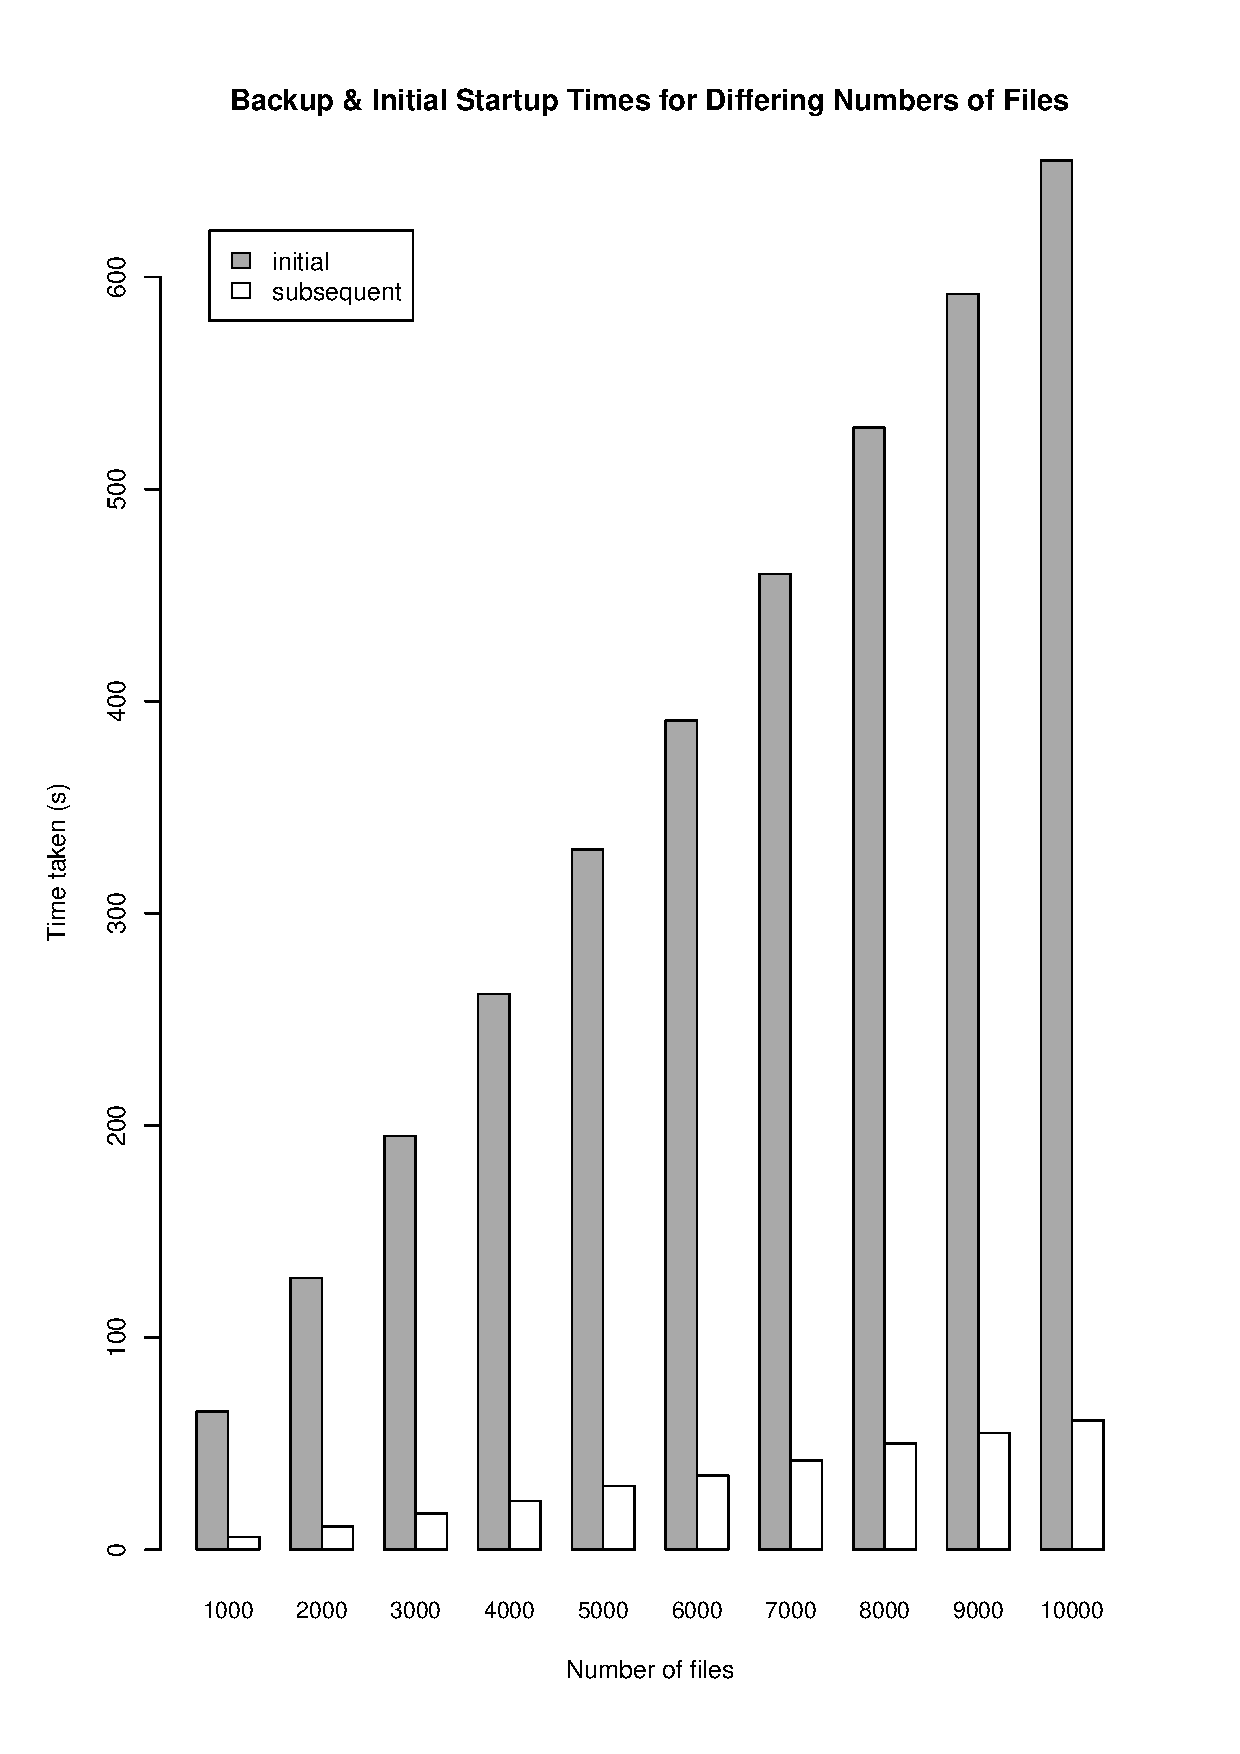
\includegraphics[width=\textwidth]{performance}
    \end{center}
    \caption{Graph showing system performance with differing numbers of files}
    \label{fig:performance-graph}
\end{figure}

Files of a small and consistent size (1KB) were intentionally used so as to
test the performance of the indexing and initial backup code, not the file
transfer speed itself, as this is dependant on network bandwidth.

Figure \ref{fig:performance-graph} shows clearly that, when acting upon files
of equal size, the performance of the system is linear (i.e. $O(n)$) in both
the initial backup and subsequent startup phases. This is a very satisfactory
result, showing that a directory tree containing 10,000 files can easily be
backed up in under 11 minutes, and subsequent startup takes only 1 minute.

\section{Evaluation}

The software produced in this project has met every requirement set out in the
specification. The end result is deemed to be a significant step towards
a viable offering by \emph{Servat, Ltd} of Nottingham, who agreed to support
this project in the initial stages and have provided a detailed evaluation.

\subsection{Servat Evaluation}

\begin{quote}
\begin{em}

    At Servat, we are mainly an accounting systems provider, installing and
    maintaining DataFile for our clients. We also resell a remote backup
    system, however, called Vembu. This is re-branded as our own product,
    DataSquirrel. DataSquirrel backs up customer data over the internet to
    a server in the cloud.

    The software Rob has produced is of a standard we would consider marketing
    as an in-house alternative to our DataSquirrel product. There are, however,
    a number of things which prevent us from doing so.
    
    Firstly, the backup system does not support Windows operating systems,
    which is a definite must in our customer environments, which are almost
    entirely Windows-based. Also, the backups themselves are not encrypted,
    which, when dealing with sensitive accounting data, would also be required.
    Finally, the installation process is somewhat complex, and would not be
    suitable for distribution to customers as-is. This would need to be refined
    before the software could be realistically used in a commercial setting.

    Aside from these issues, the software is generally well produced and
    professional. It fulfils every requirement in the specification which was
    written at the beginning of the project, and performs well in all areas. In
    particular, the web interface is well designed and intuitive, which would
    allow less technical personnel to recover files without contacting us
    unnecessarily. All-in-all, an impressive piece of work!

\end{em}
\end{quote}

\subsection{Methodology}

As described in section \ref{sec:implementation-methodology}, this project was
developed using an \emph{evolutionary prototyping} methodology. Upon
reflection, this methodology allowed for freedom in the development process,
and was extremely valuable when refining the system architecture.

Despite having only limited development experience to apply, the author
considers this methodology to be very effective, enforcing good design
principles at every step of the way. Though the design was drastically
re-considered in the early stages of the project's life, the knowledge that
each prototype fed into the next iteration encourages the developer to adhere
to so-called ``good'' design principles, making use of reusable modules and
abstracted code.

Ultimately, this has led to a well-designed, extensible system, upon which the
features discussed in sections \ref{sec:specification-evolution} and
\ref{sec:summary-further} may be developed.
